%==============================================================================
% Sjabloon poster bachproef
%==============================================================================
% Gebaseerd op document class `a0poster' door Gerlinde Kettl en Matthias Weiser
% Aangepast voor gebruik aan HOGENT door Jens Buysse en Bert Van Vreckem

\documentclass[a0,portrait]{hogent-poster}

% Info over de opleiding
\course{Bachelorproef}
\studyprogramme{toegepaste informatica}
\academicyear{2023-2024}
\institution{Hogeschool Gent, Valentin Vaerwyckweg 1, 9000 Gent}

% Info over de bachelorproef
\title{Vergelijkende studie van render cyclussen
    in SwiftUI: Impact op performance,
    rendering en lifecycles.}
\author{Wannes De Tollenaere}
\email{wannes.detollenaere@student.hogent.be}
\supervisor{Steven Van Impe}
\cosupervisor{Dennis Litjens (VRT)}

% Indien ingevuld, wordt deze informatie toegevoegd aan het einde van de
% abstract. Zet in commentaar als je dit niet wilt.
\specialisation{Mobile en Enterprise developer}
\keywords{SwiftUI, Render Cyclussen, Dataoverdracht, View-Rendering}

\begin{document}

\maketitle

\begin{abstract}
Dit onderzoek analyseert de prestaties bij gegevensoverdracht en de impact van gegevensoverdracht op rendercycli. Experimenten hebben inzichten getoond in verschillende gegevensoverdrachtssituaties. Aanbevelingen voor het ontwerpen van efficiënte gebruikersinterfaces zijn gedaan op basis van de resultaten die uit de experimenten gevloeid zijn. De onderzoeksvraag die in deze proef beantwoord is: Hoe beïnvloeden diverse gegevensoverdrachtsmethoden de prestaties en rendering van SwiftUI views, en hoe kunnen deze bevindingen worden gebruikt voor het ontwerpen van efficiënte gebruikersinterfaces? Deze vraag is beantwoord door diverse aanbevelingen te doen zodat ontwikkelaars deze methoden efficiënt kunnen gebruiken. 
\end{abstract}

\begin{multicols}{2} % This is how many columns your poster will be broken into, a portrait poster is generally split into 2 columns

\section{Introductie}
Dit onderzoek richt zich op het analyseren van data-overdrachtsmethoden binnen swiftUI, een modern framework van Apple dat een declaratieve programmeerstijl hanteert voor het ontwerpen en bouwen van gebruikersinterfaces. SwiftUI stelt ontwikkelaars in staat om snel aantrekkelijke en responsieve apps te maken, wat een verbetering betekent ten opzichte van het oudere UIKit. De focus ligt op de impact van rendercycli op de prestaties en rendering in SwiftUI-toepassingen, met specifieke aandacht voor efficiënte en reactieve gegevensoverdracht. Het doel van het onderzoek is om de meest efficiënte methoden voor gegevensoverdracht te identificeren door de invloed op geheugengebruik, CPU-gebruik en laadtijd van SwiftUI-weergaven te evalueren.

\section{Experimenten}
De experimenten die in dit onderzoek zijn uitgevoerd, omvatten verschillende scenario's van gegevensoverdracht binnen SwiftUI-toepassingen. De drie hoofdsituaties die werden getest zijn:
\newline \textbf{Gegevensoverdracht naar één child view:} In dit experiment werd getest hoe de gegevensoverdracht naar een enkele onderliggende weergave de prestaties beïnvloedt. Dit scenario is representatief voor eenvoudige toepassingen waarbij een beperkte hoeveelheid gegevens naar één specifieke weergave moet worden gestuurd.
\newline \textbf{Gegevensoverdracht naar meerdere child views in een normale lijst:} Dit experiment richtte zich op het testen van de prestaties wanneer gegevens worden overgedragen naar meerdere onderliggende weergaven binnen een traditionele lijststructuur. Deze situatie is typisch voor toepassingen die meerdere elementen tegelijkertijd moeten weergeven en bijwerken.
\newline \textbf{Gegevensoverdracht naar meerdere child views in een lazy lijst:} In dit scenario werd de gegevensoverdracht getest naar meerdere onderliggende weergaven binnen een lazy lijst. Een lazy lijst laadt elementen pas wanneer ze in beeld komen, wat efficiëntie kan verhogen bij het werken met grote datasets.

\subsection{Inzichten}
De tests hebben waardevolle inzichten opgeleverd met betrekking tot de prestaties en rendering van views in verschillende gegevensoverdrachtssituaties. Specifieke resultaten tonen aan hoe elke methode presteert op het gebied van geheugengebruik, CPU-gebruik en laadtijd van weergaven. Deze bevindingen zijn cruciaal voor het begrijpen van de efficiëntie van verschillende overdrachtsmethoden en dragen bij aan het identificeren van de meest effectieve benadering voor het verbeteren van de gebruikerservaring in SwiftUI-toepassingen.

\section{Sectie met figuur}
In deze flowchart wordt kort uitgebeeld hoe een render wordt getriggerd binnen het onderzoek. De stappen omvatten het initialiseren van de app met data, het wijzigen van de kleur van een string door op een knop te drukken om zo een dataverandering te triggeren, en het observeren van de rendercycli en performance trackers. Hierbij is gebruik gemaakt van de Xcode Profiler om de performance en de rendercycli bij te houden. De verdere analyse en conclusie van de resultaten zijn gedaan aan de hand van een opgemaakte tabel waarin de resultaten duidelijk af te lezen zijn.
\begin{center}
  \captionsetup{type=figure}
  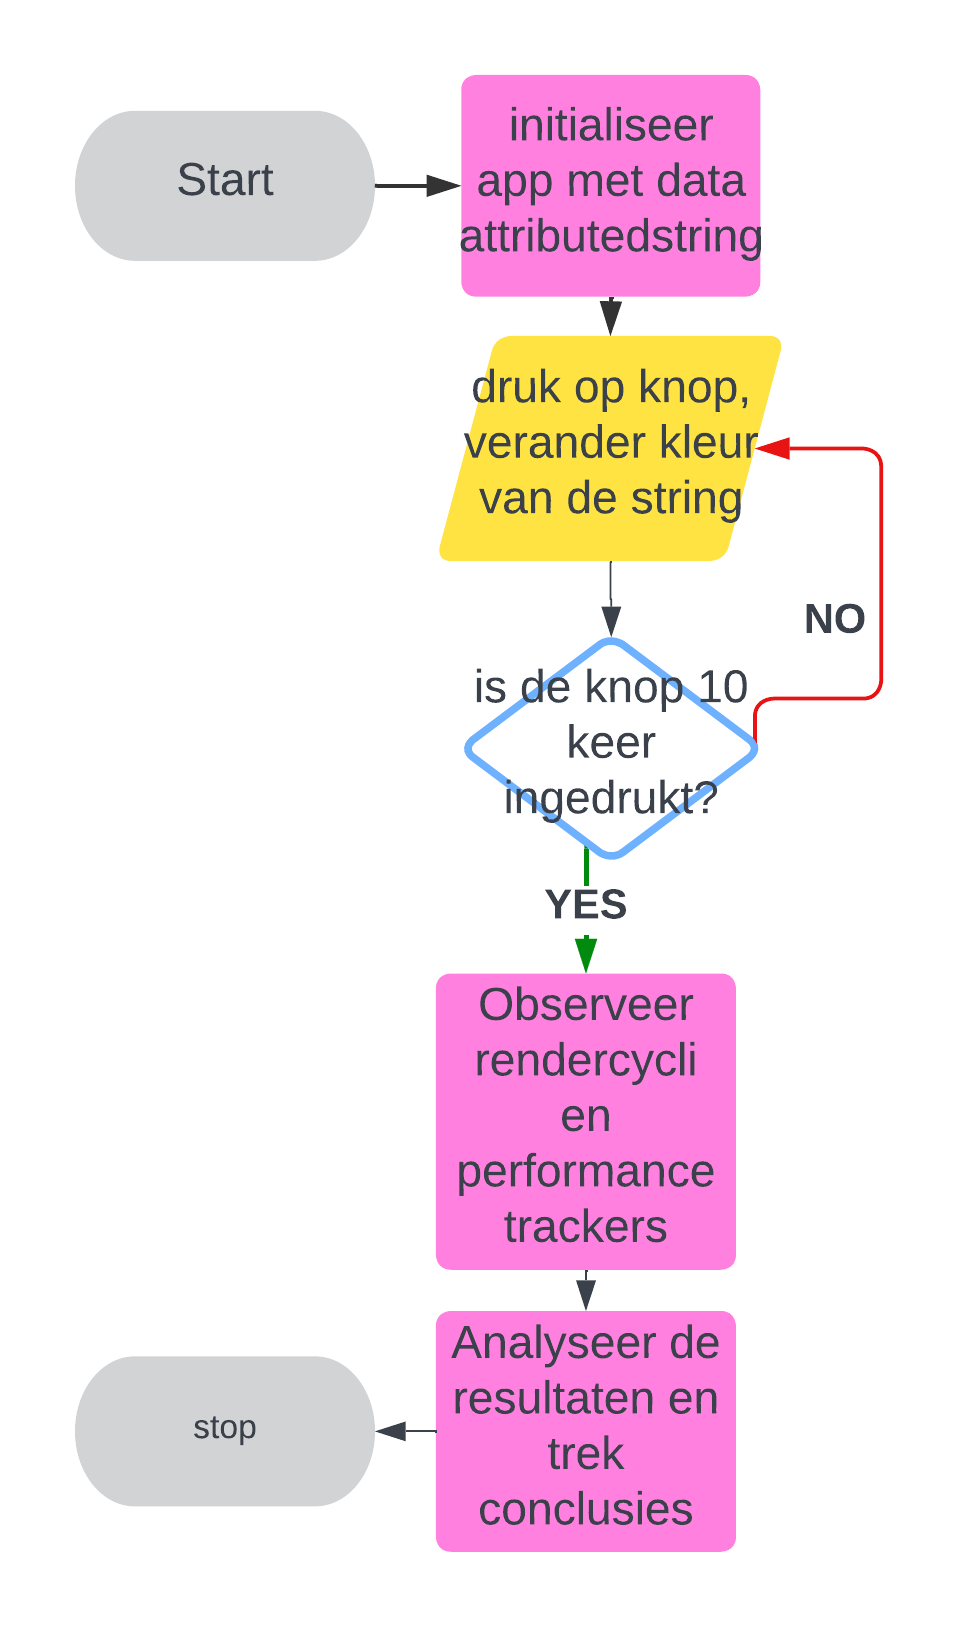
\includegraphics[width=0.5\linewidth]{flowchart}
  \captionof{figure}{flowchart van het testprocess}
\end{center}


\section{Conclusies}
Door deze methoden strategisch te kiezen op basis van de hieronder beschreven performance en efficiëntie kunnen ontwikkelaars goed presterende en responsieve gebruikersinterfaces in SwiftUI ontwerpen.\newline

\textbf{EnvironmentObject} is geschikt voor scenario’s waar een balans tussen prestaties en vernieuwingstijden belangrijk is. Het biedt efficiënte gegevensoverdracht met een lage CPU-belasting. Het kan worden gekozen voor algemene doeleinden en grotere applicaties waar meerdere subviews gegevens moeten delen.

\textbf{ObservableObject} is ideaal wanneer snelle vernieuwingstijden cruciaal zijn, ondanks de hogere CPU-belasting. Het kan worden gebruikt in scenario’s waar snelle responstijden cruciaal zijn, zoals bij real-time data updates.

\textbf{Binding} moet vermeden worden in complexe UI’s met meerdere subviews vanwege de hoge CPU-belasting en frequente updates. Het en Observable moeten vermeden worden in complexe of prestatiekritieke delen van de applicatie om inefficiënties te voorkomen.

\textbf{Observable} is minder efficiënt in termen van vernieuwingstijden en moet alleen worden gebruikt wanneer specifieke voordelen van deze methode nodig zijn.

\section{Toekomstig onderzoek}
In toekomstig onderzoek zou verder kunnen onderzocht worden naar hoe verschillende state management-technieken de ontwikkelingstijd en het onderhoud van SwiftUI-apps beïnvloeden, inclusief aspecten zoals codecomplexiteit, testbaarheid en gemak van iteratie. Zo kan er nog een betere aanbeveling gedaan worden over welke methoden het best zouden gebruikt worden in verschillende scenario's.

\end{multicols}
\end{document}